\documentclass[11pt,a4paper]{article}
\usepackage[utf8]{inputenc}
\usepackage[portuguese]{babel}
\usepackage{amsmath}
\usepackage{amssymb}
\usepackage{graphicx}
\usepackage{listings}
\usepackage{xcolor}
\usepackage{float}
\usepackage{geometry}
\usepackage{fancyhdr}
\usepackage{hyperref}
\usepackage{array}

% Figuras geradas por scripts/gerar_grafos.py ficam em relatorio/figuras/
\graphicspath{{../figuras/}}

\geometry{left=1.5cm,right=1.5cm,top=1.5cm,bottom=1.5cm}
\setlength{\parskip}{0.3em}
\setlength{\floatsep}{6pt}
\setlength{\textfloatsep}{8pt}
\pagestyle{fancy}

% Configuracao de cores para codigo
\definecolor{codegreen}{rgb}{0,0.6,0}
\definecolor{codegray}{rgb}{0.5,0.5,0.5}
\definecolor{codepurple}{rgb}{0.58,0,0.82}
\definecolor{backcolour}{rgb}{0.95,0.95,0.92}

\lstset{
    backgroundcolor=\color{backcolour},
    commentstyle=\color{codegreen},
    keywordstyle=\color{codepurple},
    numberstyle=\tiny\color{codegray},
    stringstyle=\color{codegray},
    basicstyle=\ttfamily\footnotesize,
    breakatwhitespace=false,
    breaklines=true,
    captionpos=b,
    keepspaces=true,
    numbers=left,
    numbersep=5pt,
    showspaces=false,
    showstringspaces=false,
    showtabs=false,
    tabsize=4,
    language=Python,
    frame=single
}

% Cabecalho e Rodape
\lhead{CC8550 --- Simulacao e Teste de Software}
\chead{Aula 04}
\rhead{2º Semestre 2025}
\cfoot{Página \thepage}

\title{
    {\Large \textbf{Simulação e Teste de Software}} \\
    {\Large \textbf{Aula 04 --- Técnicas Caixa-Branca: Critérios de Cobertura Estrutural}} \\
    \vspace{0.5cm}
    {\small Solução Completa de Exercícios}
}

\author{
    \textbf{Aluno:} Lucas Rebouças Silva \\
    \textbf{R.A.:} 22.122.048-6 \\[0.3cm]
    \textbf{Professor:} Luciano Rossi \\
    \textbf{Centro Universitário FEI} \\
    Ciência da Computação
}

\date{2º Semestre de 2025}

\begin{document}

\maketitle

\newpage
\tableofcontents
\newpage

% ============================================================================
% EXERCICIO 1
% ============================================================================
\section{Exercício 1 --- Caminhos Independentes}

\subsection{Código}

\begin{lstlisting}
def verificar(n):
    if n > 0:
        if n % 2 == 0:
            return "Par positivo"
        else:
            return "Impar positivo"
    elif n < 0:
        return "Negativo"
    else:
        return "Zero"
\end{lstlisting}

\subsection{GFC e V(G)}

\begin{figure}[H]
\centering
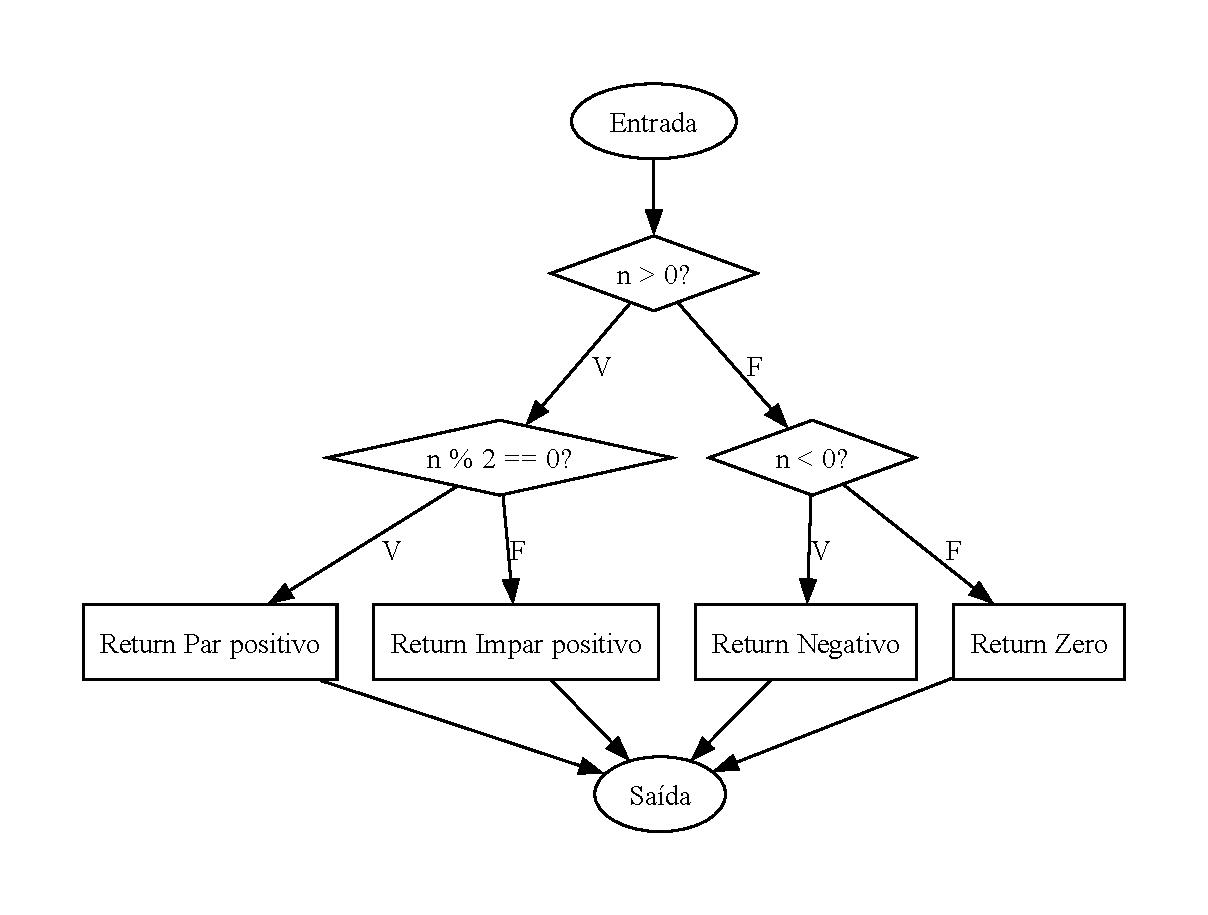
\includegraphics[width=0.7\textwidth]{ex1_gfc}
\caption{GFC Exercício 1}
\end{figure}

$V(G) = 3$. Caminhos: $n=0$ (Zero), $n=2$ (Par positivo), $n=-1$ (Negativo), $n=3$ (Impar positivo). Casos de teste: (0, Zero), (2, Par positivo), (-1, Negativo), (3, Impar positivo).

\newpage

% ============================================================================
% EXERCICIO 2
% ============================================================================
\section{Exercício 2 --- Cobertura de Comandos e Ramos}

\subsection{Código}

\begin{lstlisting}
def classificar(x):
    if x > 100:
        return "Alto"
    if x > 50:
        return "Medio"
    return "Baixo"
\end{lstlisting}

\begin{figure}[H]
\centering
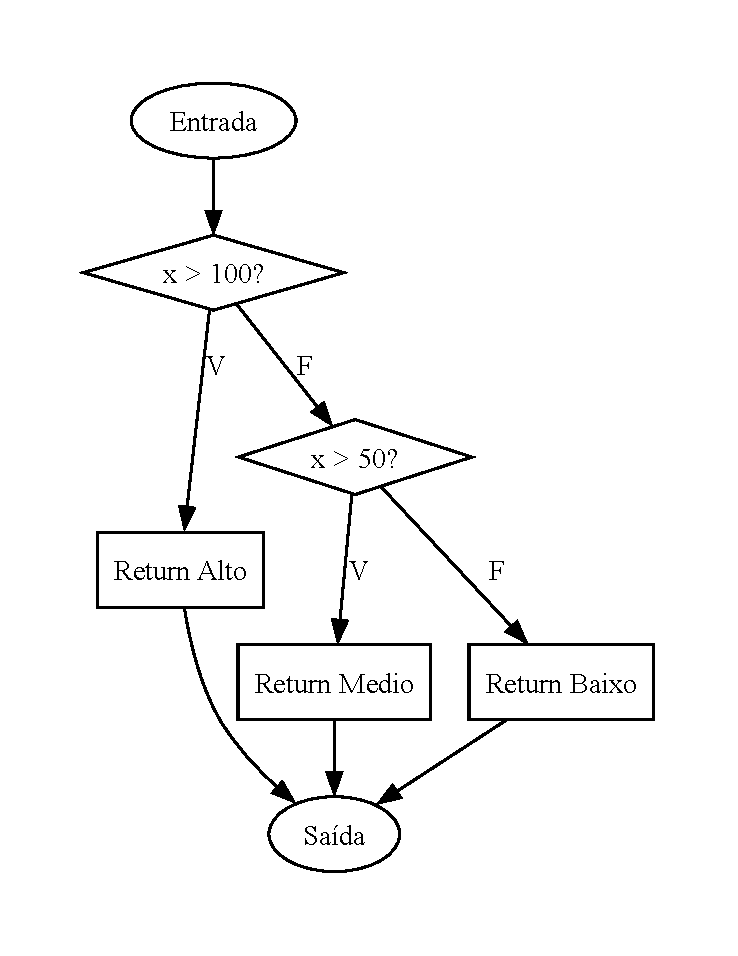
\includegraphics[width=0.65\textwidth]{ex2_gfc}
\caption{GFC Exercício 2}
\end{figure}

$V(G) = 3$. C0 e C1: 3 testes — (150, Alto), (75, Medio), (25, Baixo).

\newpage

% ============================================================================
% EXERCICIO 3
% ============================================================================
\section{Exercício 3 --- Cobertura de Condição}

\subsection{Código}

\begin{lstlisting}
def acesso(idade, membro):
    if idade >= 18 and membro:
        return "Permitido"
    return "Negado"
\end{lstlisting}

\begin{figure}[H]
\centering
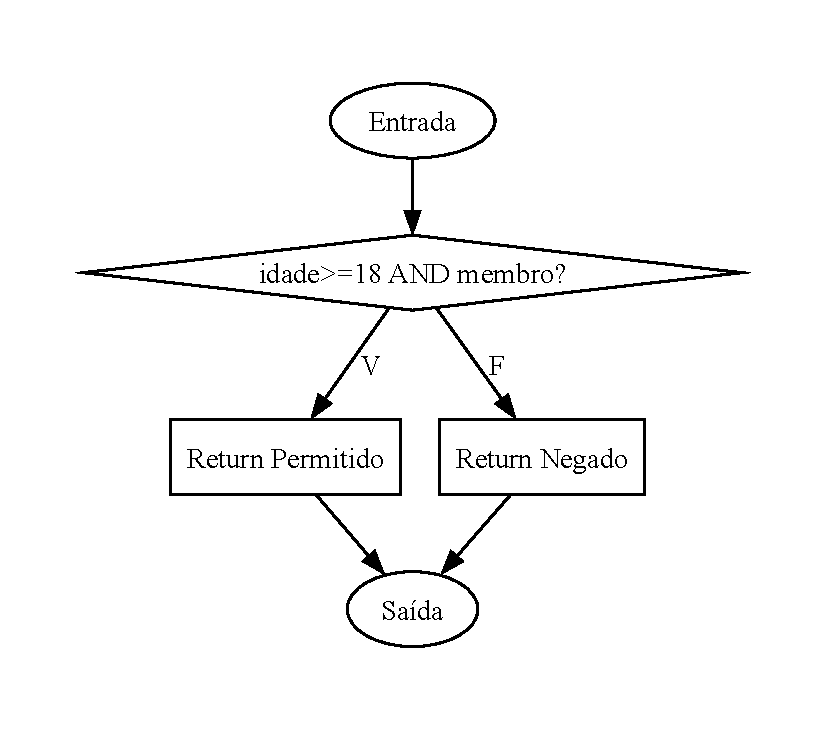
\includegraphics[width=0.55\textwidth]{ex3_gfc}
\caption{GFC Exercício 3}
\end{figure}

$V(G) = 2$. Condição: $(idade \geq 18) \land membro$. C1: 2 testes (25, True $\to$ Permitido; 20, False $\to$ Negado). CC: 4 testes para cobrir as 4 combinações (25/T, 25/F, 17/T, 17/F $\to$ Permitido só no primeiro).

\newpage

% ============================================================================
% EXERCICIO 4
% ============================================================================
\section{Exercício 4 --- Teste de Ciclo}

\subsection{Código}

\begin{lstlisting}
def somar_ate(n):
    soma = 0
    for i in range(n):
        soma += i
    return soma
\end{lstlisting}

\begin{figure}[H]
\centering
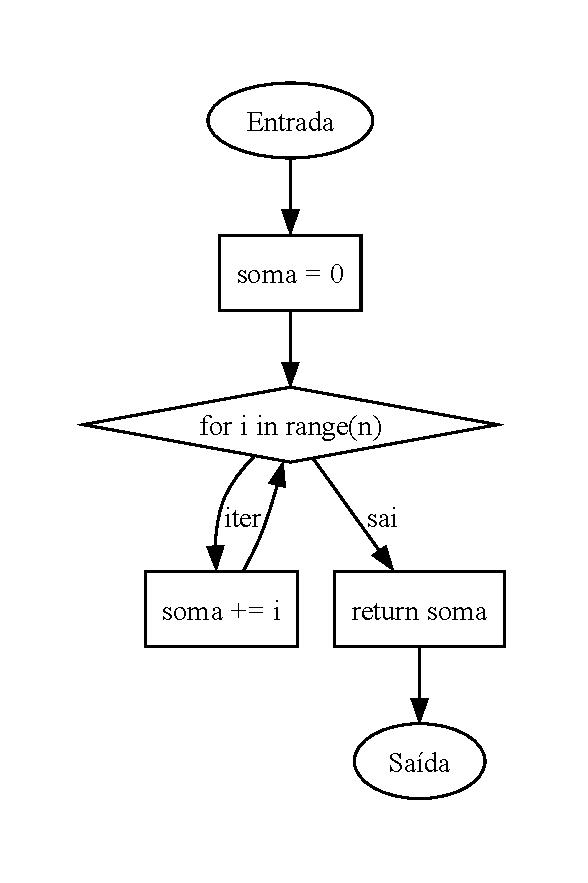
\includegraphics[width=0.6\textwidth]{ex4_gfc}
\caption{GFC Exercício 4}
\end{figure}

$V(G) = 2$. Teste de ciclo: 0, 1 e várias iterações. Casos: $n=0\to 0$, $n=1\to 0$, $n=2\to 1$, $n=5\to 10$, $n=10\to 45$.

\newpage

% ============================================================================
% EXERCICIO 5
% ============================================================================
\section{Exercício 5 --- Teste de Ciclo Aninhado}

\subsection{Código}

\begin{lstlisting}
def percorrer_matriz(m, n):
    posicoes = []
    for i in range(m):
        for j in range(n):
            posicoes.append((i, j))
    return posicoes
\end{lstlisting}

\begin{figure}[H]
\centering
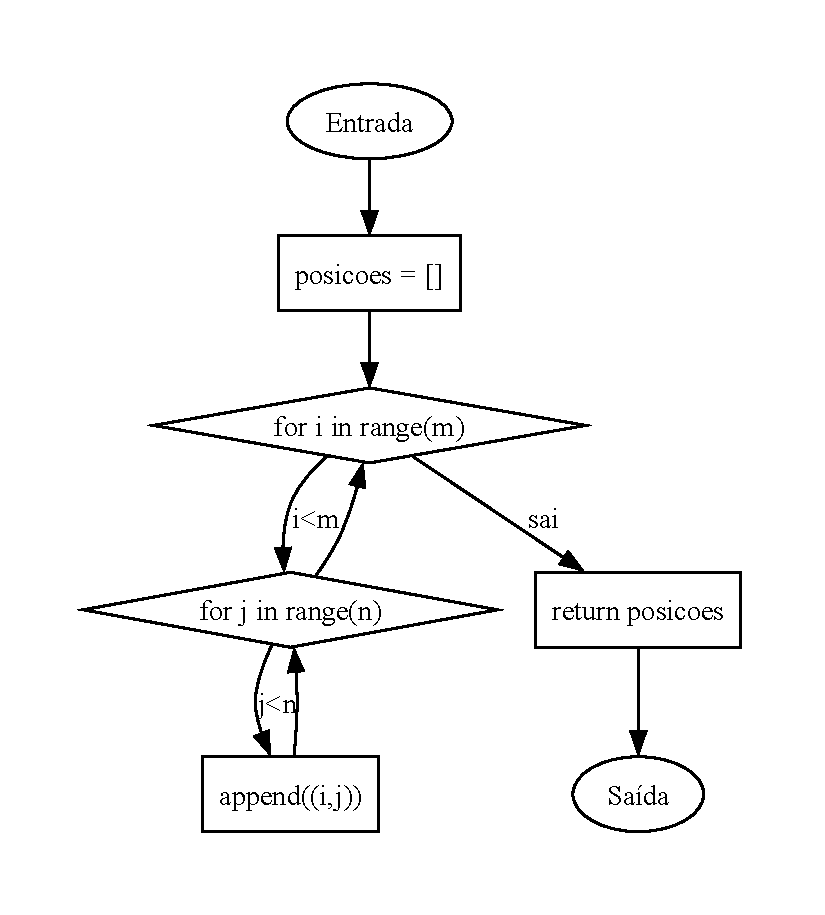
\includegraphics[width=0.6\textwidth]{ex5_gfc}
\caption{GFC Exercício 5}
\end{figure}

$V(G) = 3$. Iterações totais: $m \times n$. Cenários: (0,0)$\to$0; (3,0),(0,3)$\to$0; (1,3),(3,1)$\to$3; (2,3)$\to$6; (4,5)$\to$20.

\newpage

% ============================================================================
% EXERCICIO 6
% ============================================================================
\section{Exercício 6 --- Teste Completo (Integrador)}

\subsection{Código}

\begin{lstlisting}
def analisar(numeros):
    total = 0
    for n in numeros:
        if n > 0 and n % 2 == 0:
            total += n
        elif n < 0:
            total -= 1
        else:
            continue
    if total > 10:
        return "Acima"
    return "Abaixo"
\end{lstlisting}

\begin{figure}[H]
\centering
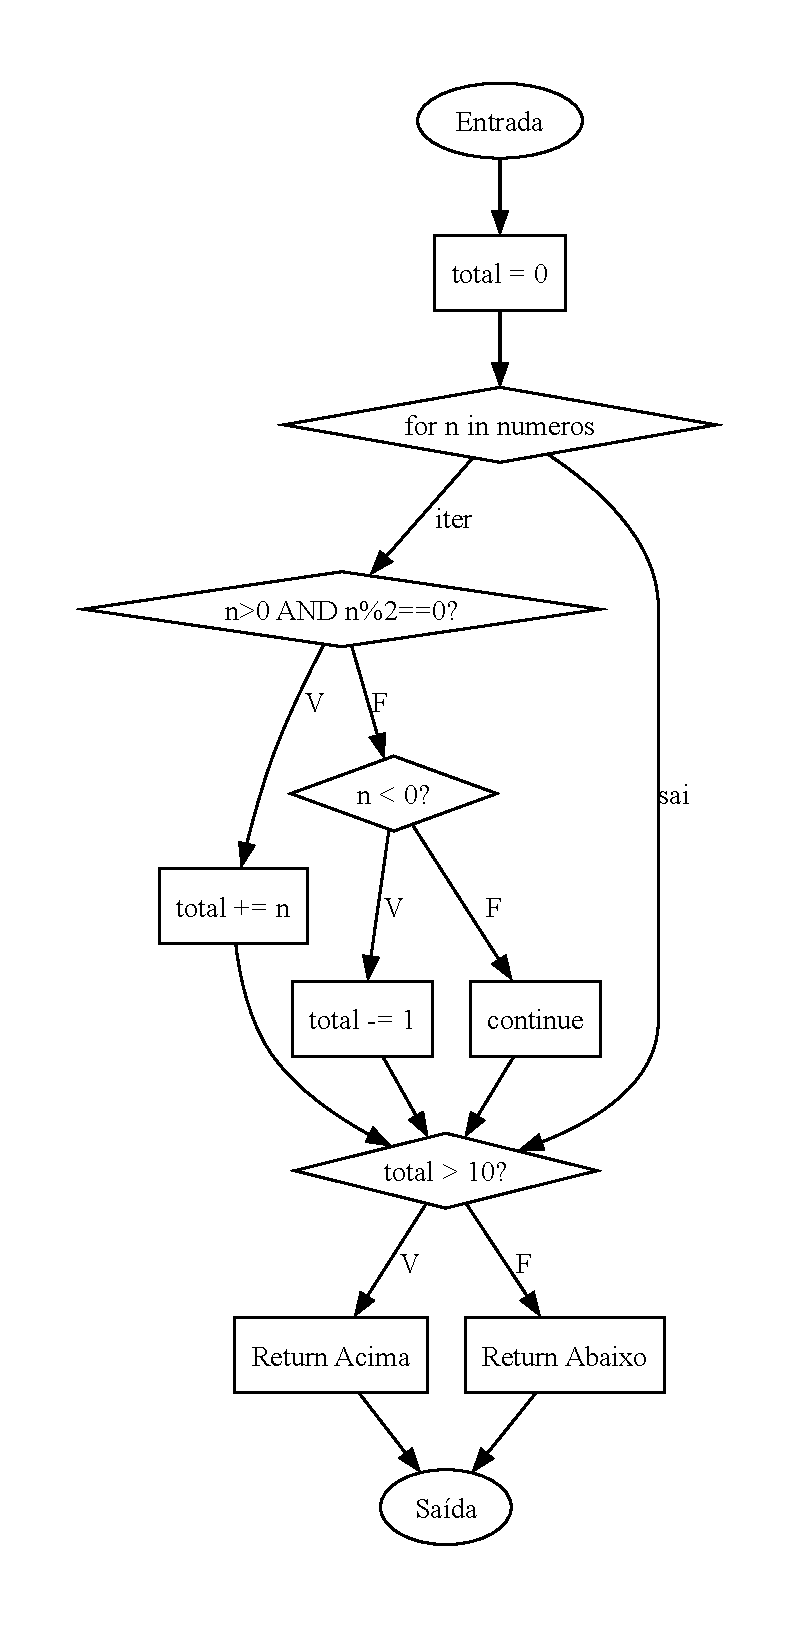
\includegraphics[width=0.4\textwidth]{ex6_gfc}
\caption{GFC Exercício 6}
\end{figure}

$V(G) = 5$. C0/C1: cobrir total+=n, total-=1, continue, return Acima/Abaixo e o desvio de laço (entrada/saída do \texttt{for}). Casos (resumo): []$\to$Abaixo; [6]$\to$Abaixo; [6,8]$\to$Acima; [1],[-2]$\to$Abaixo; [4,3,8],[6,-2,8],[0,6,8]$\to$Acima; [2,4,1]$\to$Abaixo. Def-uso \texttt{total}: def(2,5,7), use(10,11-12).

\newpage

% ============================================================================
% EXERCICIO 7
% ============================================================================
\section{Exercício 7 --- Fluxo de Dados}

\subsection{Código}

\begin{lstlisting}
def desconto(preco, cliente_vip):
    total = preco                    # linha 2: def(total)
    if cliente_vip:                  # linha 3: use(cliente_vip)
        desconto_valor = preco * 0.2 # linha 4: def(desconto_valor)
        total = preco - desconto_valor # linha 5: def(total)
    if total < 50:                   # linha 6: use(total)
        total = 50                   # linha 7: def(total)
    return total                     # linha 8: use(total)
\end{lstlisting}

\begin{figure}[H]
\centering
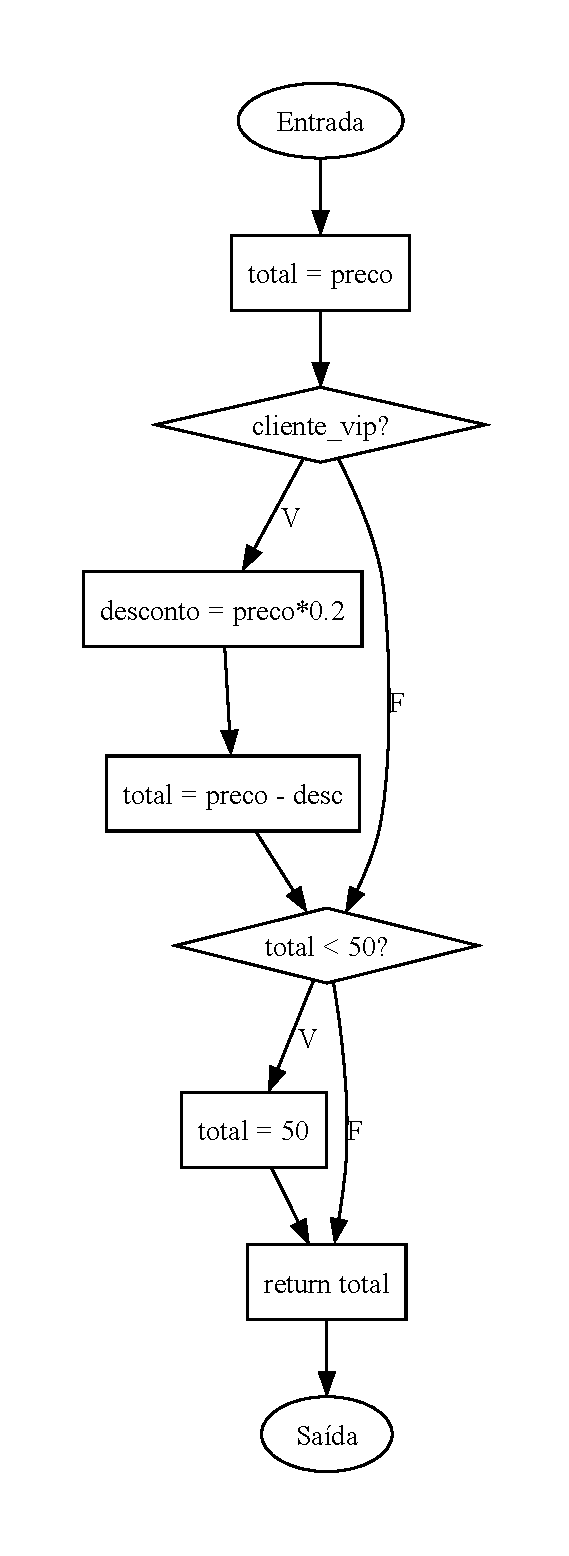
\includegraphics[width=0.35\textwidth]{ex7_gfc}
\caption{GFC Exercício 7 (def-uso)}
\end{figure}

$V(G) = 3$. As decisões são o teste de \texttt{cliente\_vip} e o teste de \texttt{total < 50}, mais o caminho sequencial base. A análise de fluxo de dados considera as variáveis \texttt{total} (definições nas linhas 2, 5 e 7; usos nas linhas 6 e 8) e \texttt{desconto\_valor} (definição na linha 4 e uso na linha 5). Uma suíte enxuta de testes que explora os caminhos com e sem cliente VIP, bem como valores acima e abaixo do piso de R\$50, é suficiente para cobrir todos os pares def-uso relevantes (All-Defs e All-Uses).

\section{Resumo e Conclusões}

Hierarquia: C0 $\leq$ C1 $\leq$ CC $\leq$ caminhos; All-Defs/All-Uses complementam. Resumo: 7 exercícios, V(G) total 19, 39+ casos de teste. Recomendações: atingir no mínimo C1; usar CC em condições compostas; All-Uses em funções críticas.

\end{document}
